\section{Método}

\subsection{Datos}
Para entrenar nuestras redes y probar los ataques adversarios y las defensas contra ellos, se emplearon las dos bases de datos más sencillas para procesamiento de imágenes: MNIST y CIFAR-10.

\subsubsection{MNIST}
La base de datos MNIST es un compendio de los dígitos del 0 al 9 en letra manuscrita con 60,000 imágenes para entrenar a distintos sistemas de procesamiento de imágenes y 10,000 imágenes para evaluarlos. Se trata de un subconjunto de imágenes de un conjunto más grande que compiló el National Institute of Standards and Technology (NIST) del Departamento de Comercio los EEUU. Las siglas MNIST database significan Modified NIST database. Es una buena base de datos para probar técnicas de aprendizaje y métodos de reconocimiento de patrones con datos del mundo real empleando un esfuerzo mínimo en preprocesamiento y formato.

De las 10,000 imágenes de evaluación, la mitad fueron escritas por estudiantes de preparatoria y la otra mitad por empleados de la oficina de censos, mientras que de las 60,000 imágenes de entrenamiento, 58,527 de los números fueron escritos por 500 estudiantes y el resto por los empleados.

El tamaño de estas imágenes en blanco y negro fue normalizado a una caja de 20x20 pixeles y se colocó su centro de masa en un campo de 28x28 \cite{lecun2010mnist}. En la Figura \ref{mnist} se muestran algunos ejemplos de estas imágenes.

\begin{figure}[h]
    \centering
    \begin{subfigure}[b]{0.4\textwidth}
        \centering
        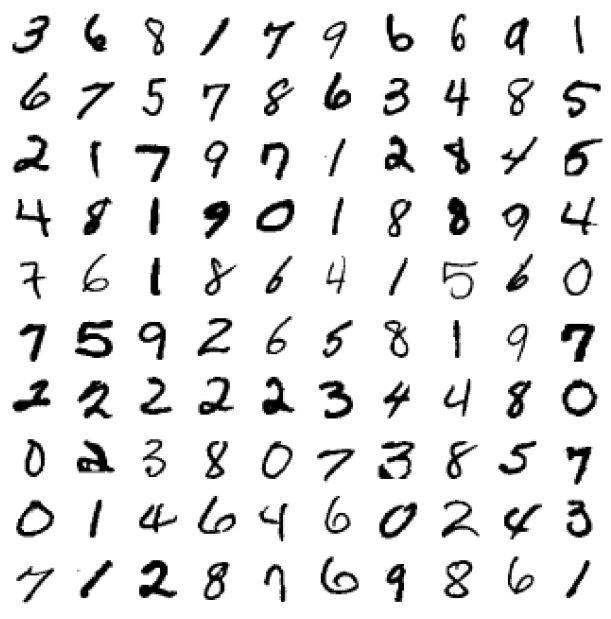
\includegraphics[width=\textwidth]{images/MNIST.png}
        \caption{Algunas imágenes del conjunto de evaluación de la base de datos MNIST \cite{Lecun98}.}
        \label{mnist1}
    \end{subfigure}
    \hspace{1cm}
    \begin{subfigure}[b]{0.45\textwidth}
        \centering
        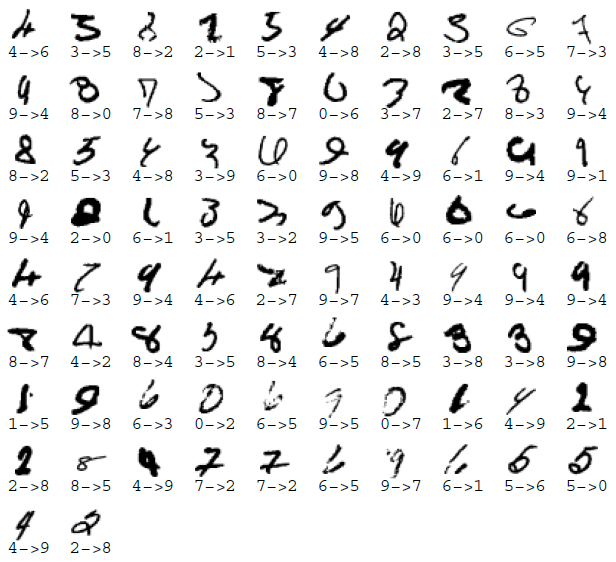
\includegraphics[width=\textwidth]{images/MNISTmiscl.png}
        \caption{82 imágenes de evaluación que LeNet-5 clasificó erróneamente \cite{Lecun98}.}
        \label{mnist2}
    \end{subfigure}
    \caption{Imágenes de MNIST.}
    \label{mnist}
\end{figure}

\subsubsection{CIFAR-10}
\cite{Krizhevsky09learningmultiple}


\subsection{Ataques}

\subsubsection{Fast Gradient Method}
\cite{goodfellow2015explaining, maybe more}

Sean $\theta$ los parámetros de un modelo, $x$ la entrada, $y$ las salidas asociadas, y $J(\theta, x, y)$ la función de costo. La función de costo se lineariza alrededor del valor actual de $\theta$. Sea $\epsilon \in \mathbb{R}^+$. Definamos la imagen adversaria 
\[\tilde{x} = x + \epsilon \eta_{\text{opt}}\]
Se puede definir $\eta_{\text{opt}}$ por el problema de optimización
\[\eta_{\text{opt}} = \operatornamewithlimits{argmax}_{\eta}\left\{ \operatorname{grad} ^\top \eta: \norm{\eta}_p< \epsilon\right\}\]
Donde $p \in \mathbb{N} \cup \{\infty\}$ y $\operatorname{grad} = \nabla_x J(\theta, x, y)$. Experimentamos con tres valores de $p$:
\begin{enumerate}[a)]
    \item $p = 1$, no lo sé, pero se encuentra en el codigo
    \item $p = 2$,
    \[\eta_{\text{opt}} = \frac{\operatorname{grad}}{\norm{\operatorname{grad}}}\]
    \item $p = \infty$,
    \[\eta_{\text{opt}} = \operatorname{sign}(\nabla_x J(\theta, x, y))\]
\end{enumerate}

\subsubsection{Carlini \& Wagner}
\cite{carlini2017evaluating} 

\subsection{Defensas}

\subsubsection{Compresión JPEG }
\cite{das2017keeping}